%!TEX root = ../SciVis.tex

 Stream tubes are similar to streamlines, they display the paths of particles in a typically three-dimensional vector field as cylindrical tubes whose cross-section size can vary to encode additional parameters.
 
 To use this technique, we must first have a three-dimensional vector field,
 time-dependent simulation, if we consider time as the third (z) dimension. 
 
 should give you a three-dimensional 'data cube'. 
 
 \begin{figure}[htbp]
 \centering
 \begin{minipage}[t]{0.48\textwidth}
 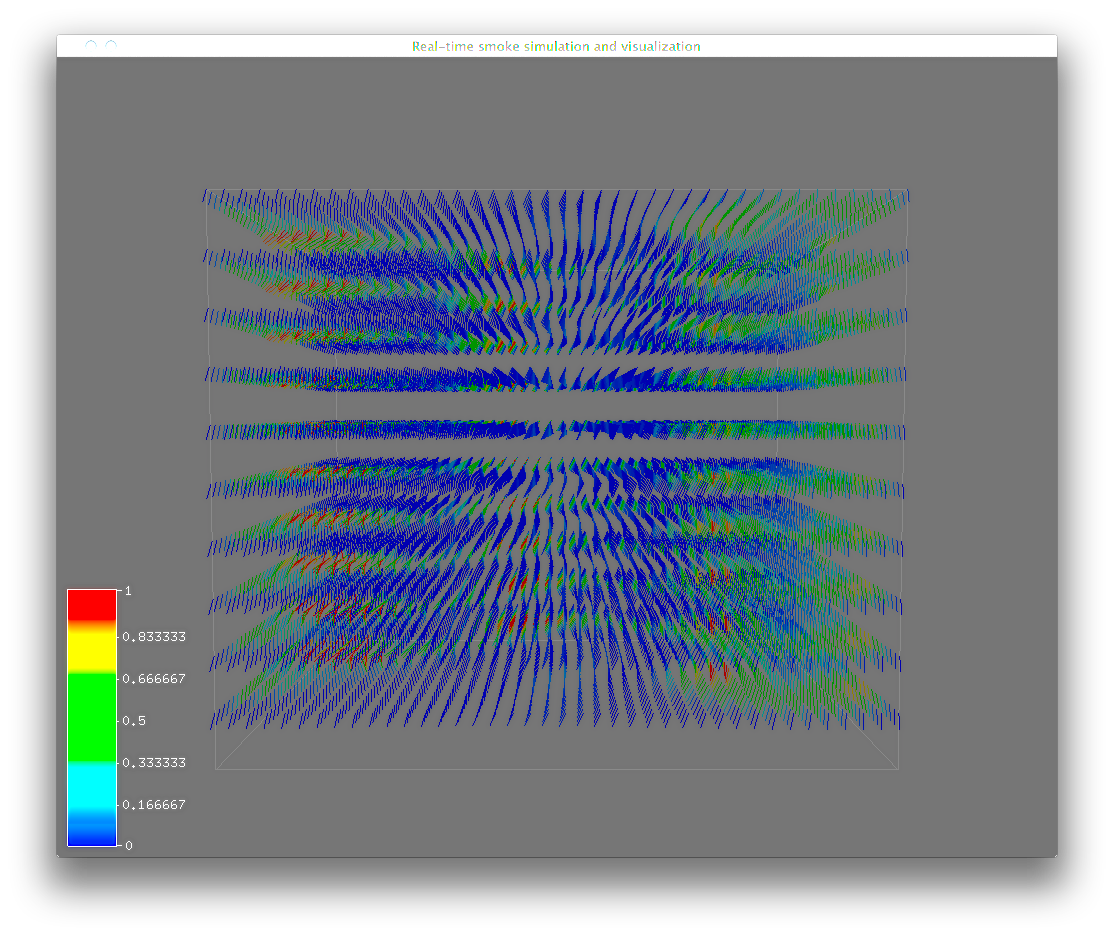
\includegraphics[height=3in]{figures/streamtubes/30datacube_bottom.png}
 \caption{}
 \label{fig:}
 \end{minipage}\hspace{.04\textwidth}%
 \begin{minipage}[t]{0.48\textwidth}
 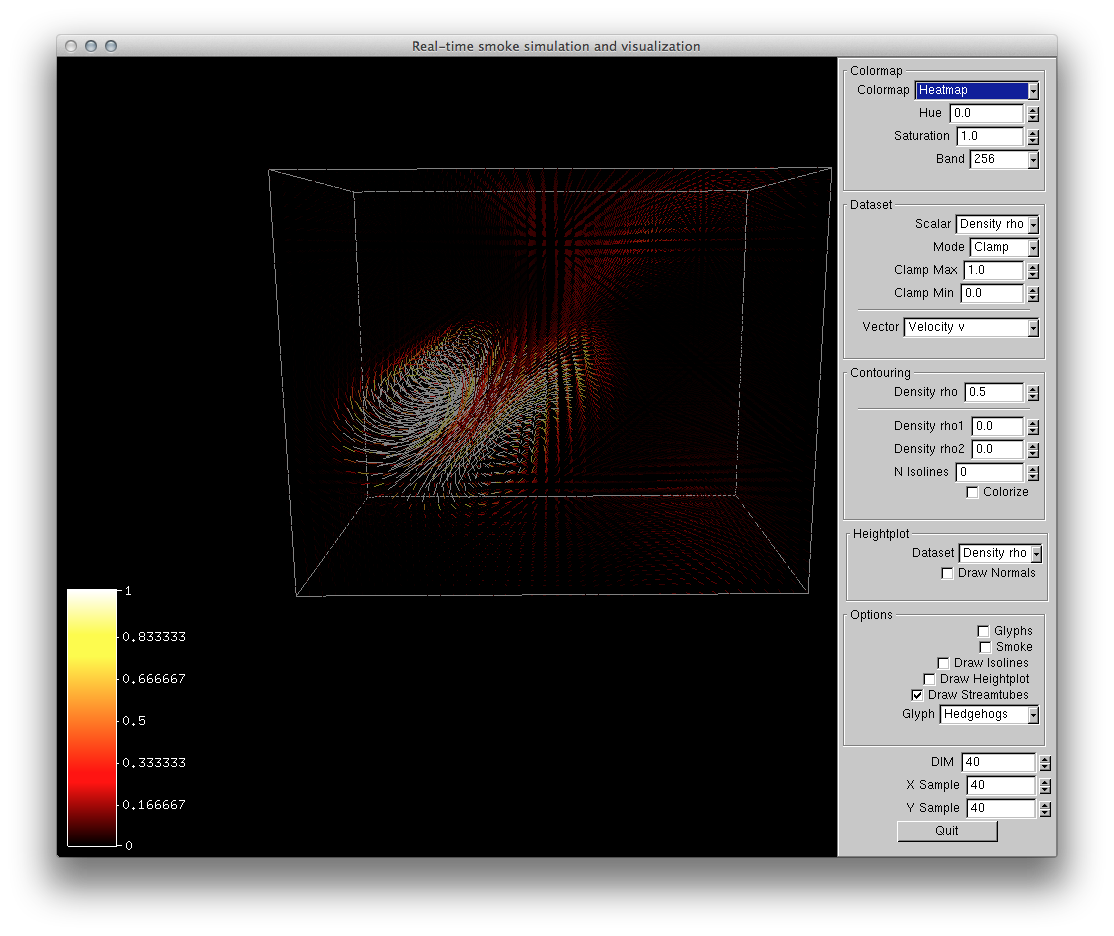
\includegraphics[height=3in]{figures/streamtubes/31datacube_front.png}
 \caption{}
 \label{fig:}
 \end{minipage}
 \end{figure}
 
 
 place (and remove) seed points in the 3D volume.
 
 control the (x,y,z) position of a seed point by means of sliders. 
 allow users to click in some point in the window. 
 
 
  accomodate three dimensions instead of two.
  
  
  
construct a stream tube geometry around it. 
asubsequent step is to use a circle sampled as a closed polyline with n points, user-controlled

 For each sample point pi along a streamline, construct such a cross-section. The cross-section should be orthogonal to the current polyline segment pi, pi+1.
 
 
 
 how to exactly place the cross-section? 
 
 a full reference frame in 3D, placed at each streamline point, which indicates the exact position and orientation of the cross-section. 
 
 get direction, local and up vector
 rotation matrix
 gets 'swept' along it
 
 
 shading and coloring of the stream tubes: use either flat or Gouraud shading, and either a constant color, 
 
 
 a color map which shows one of the scalar fields along the streamline, such as velocity vector magnitude |v| or density rho.

(diameter) of the streamtubes. 
linearly scaled to show one of the scalar field values in the simulation, such as velocity vector magnitude |v| or density rho. 
all fields muharhar



\begin{figure}[htbp]
\centering
\begin{minipage}[t]{0.48\textwidth}
        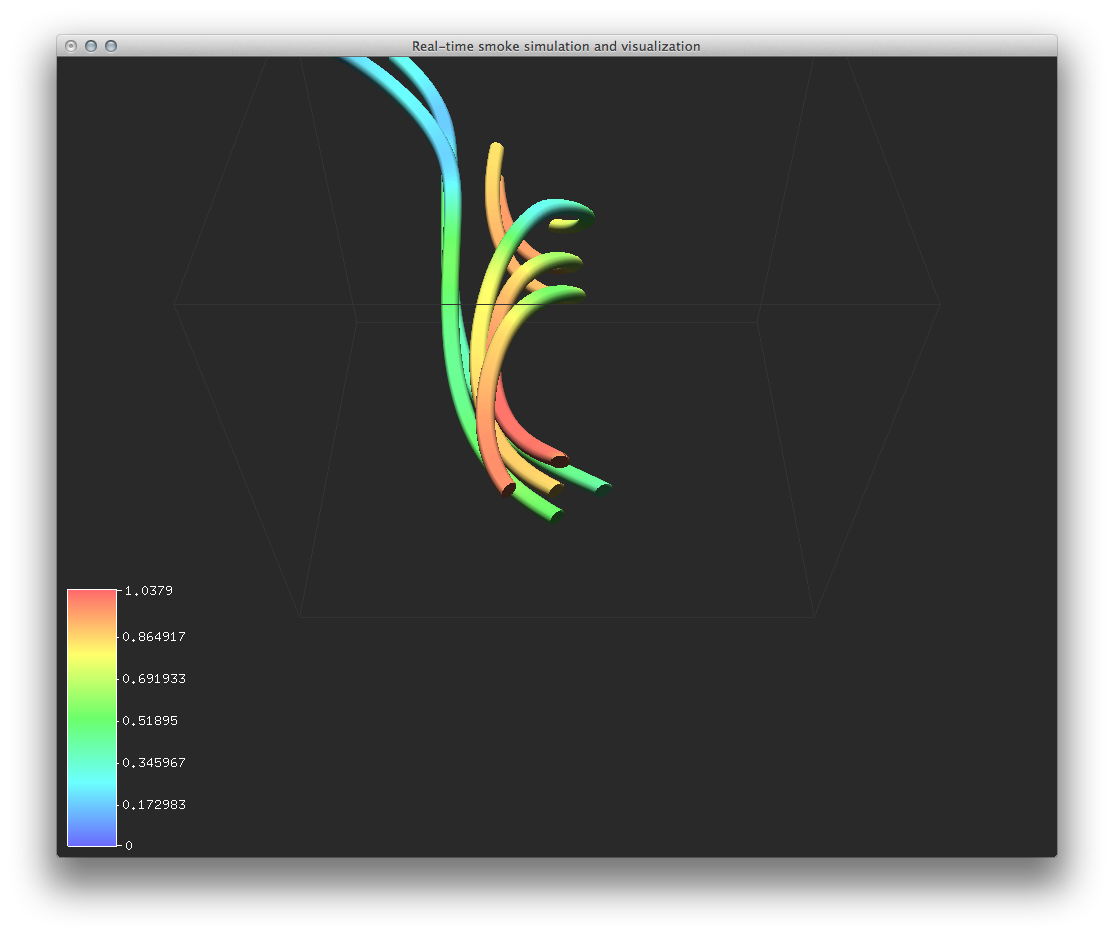
\includegraphics[height=3in]{figures/streamtubes/10tubes.png}
\caption{Hedgehog visualization of the time-dependent velocity vector field. The time-slices  shows the datacube }
\label{fig:}
\end{minipage}\hspace{.04\textwidth}%
\begin{minipage}[t]{0.48\textwidth}
    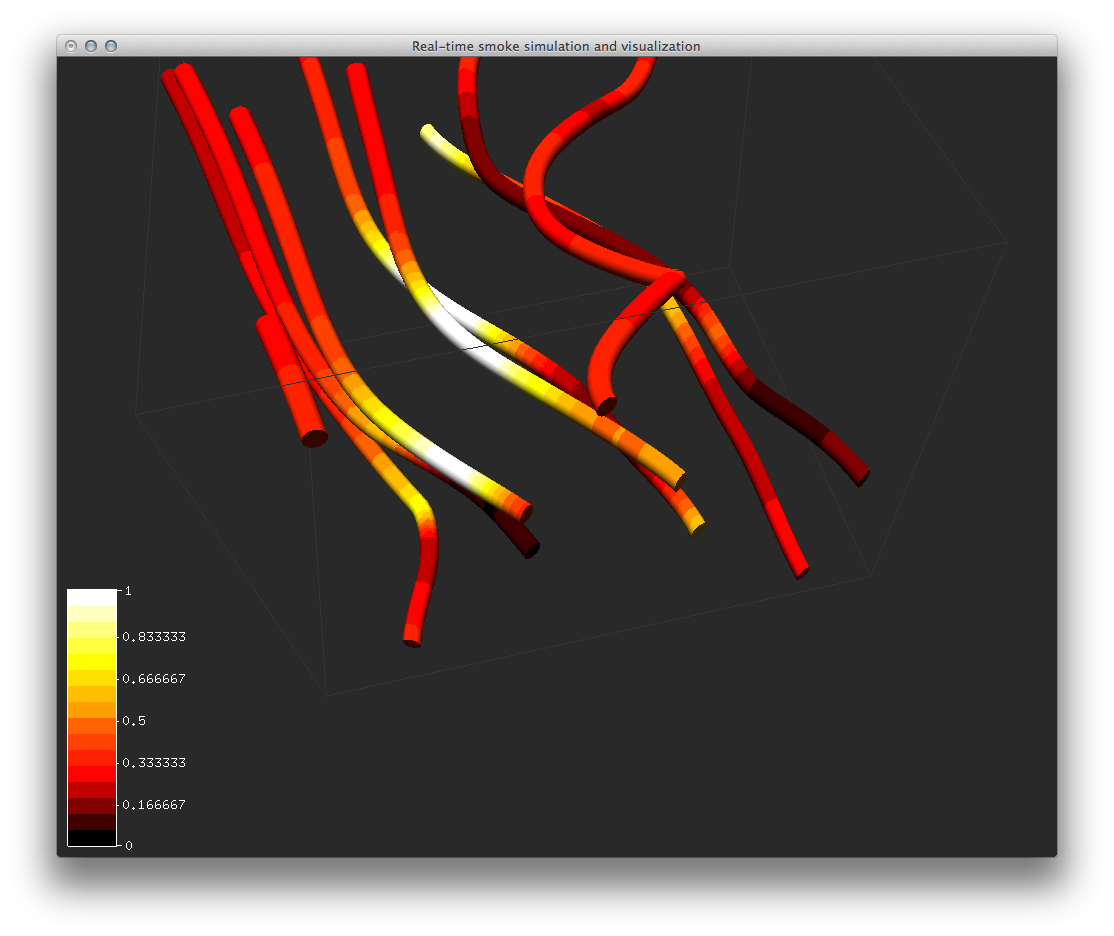
\includegraphics[height=3in]{figures/streamtubes/21banding_velodensity.png}
    \caption{}
    \label{fig:}
\end{minipage}
\end{figure}    

\begin{figure}[htbp]
\centering
\begin{minipage}[t]{0.48\textwidth}
        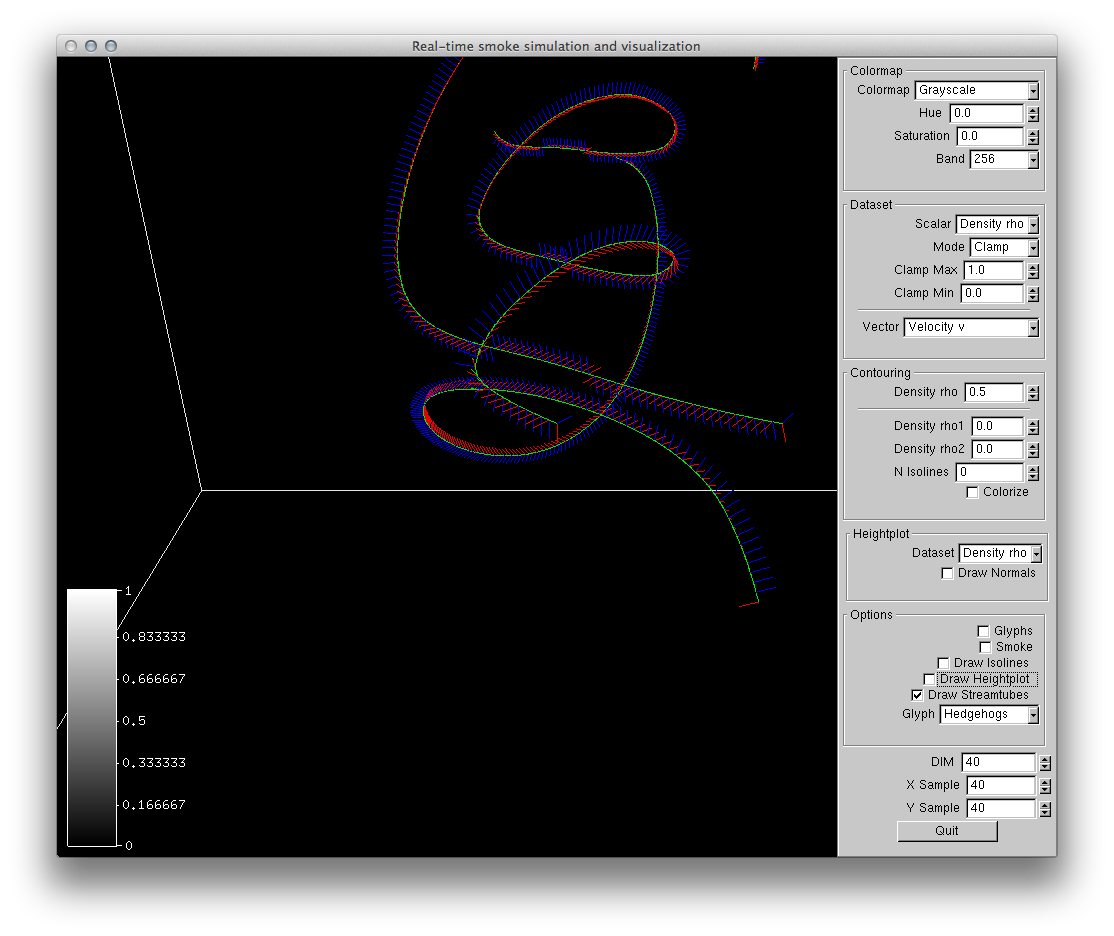
\includegraphics[height=3in]{figures/streamtubes/uvp.png}
\caption{}
\label{fig:}
\end{minipage}\hspace{.04\textwidth}%
\begin{minipage}[t]{0.48\textwidth}
               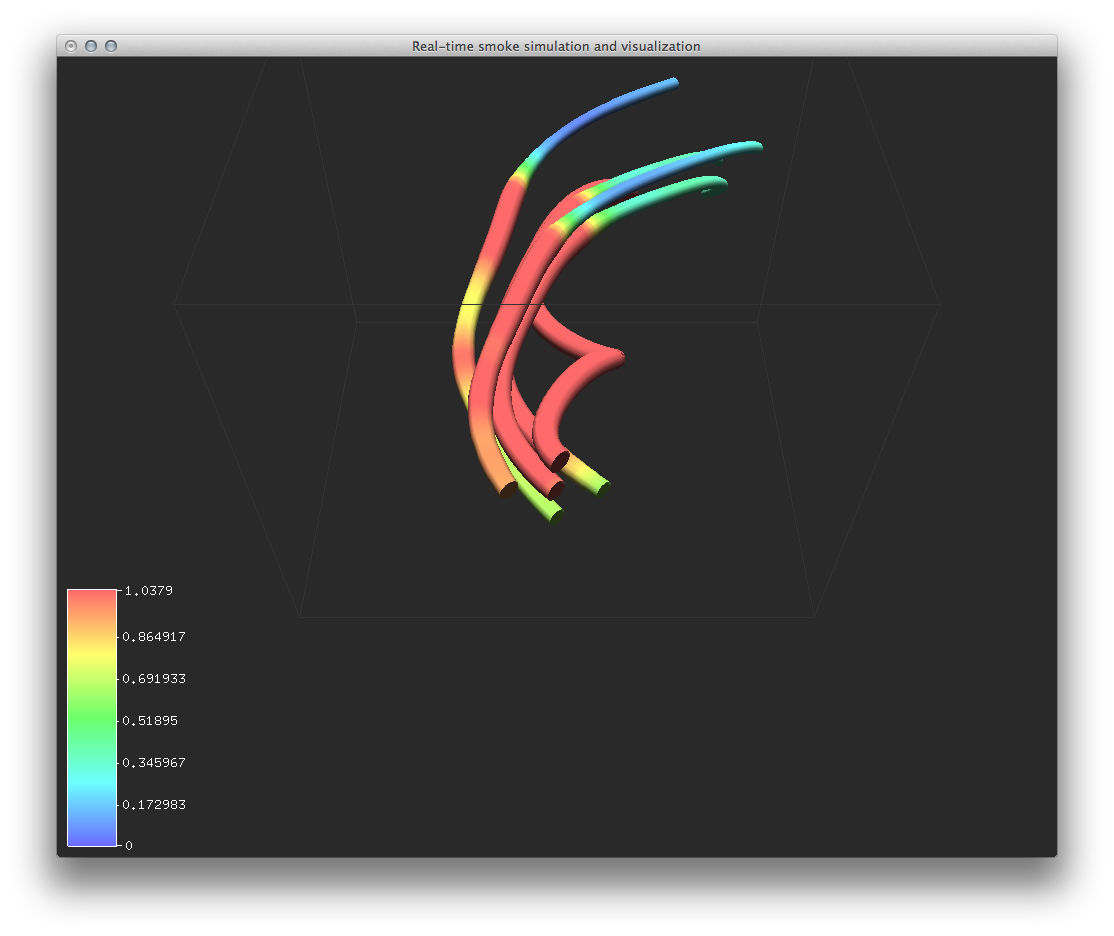
\includegraphics[height=3in]{figures/streamtubes/11thickTubes.png} 
    \caption{}
    \label{fig:}
\end{minipage}
\end{figure}



\begin{figure}[htbp]
\centering
\begin{minipage}[t]{0.48\textwidth}
        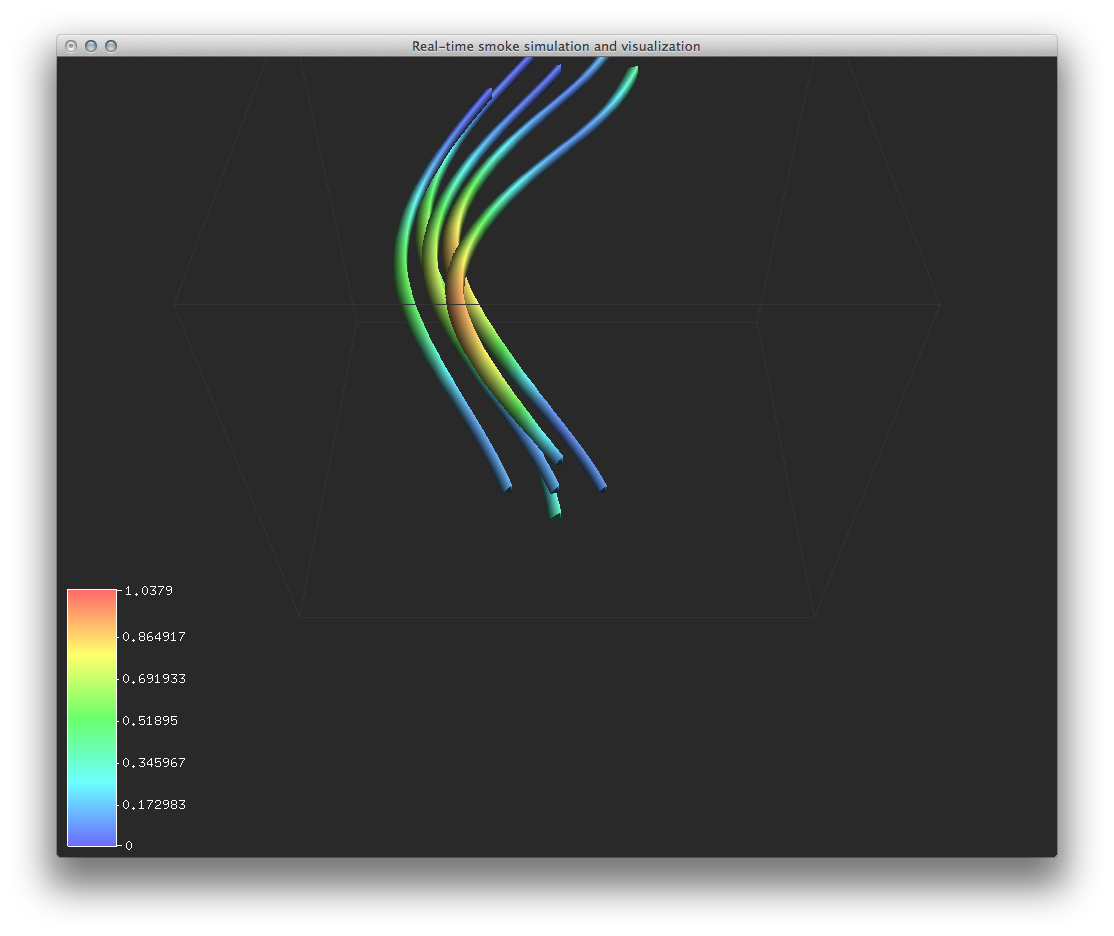
\includegraphics[height=3in]{figures/streamtubes/40threeSegments.png}
\caption{}
\label{fig:}
\end{minipage}\hspace{.04\textwidth}%
\begin{minipage}[t]{0.48\textwidth}
        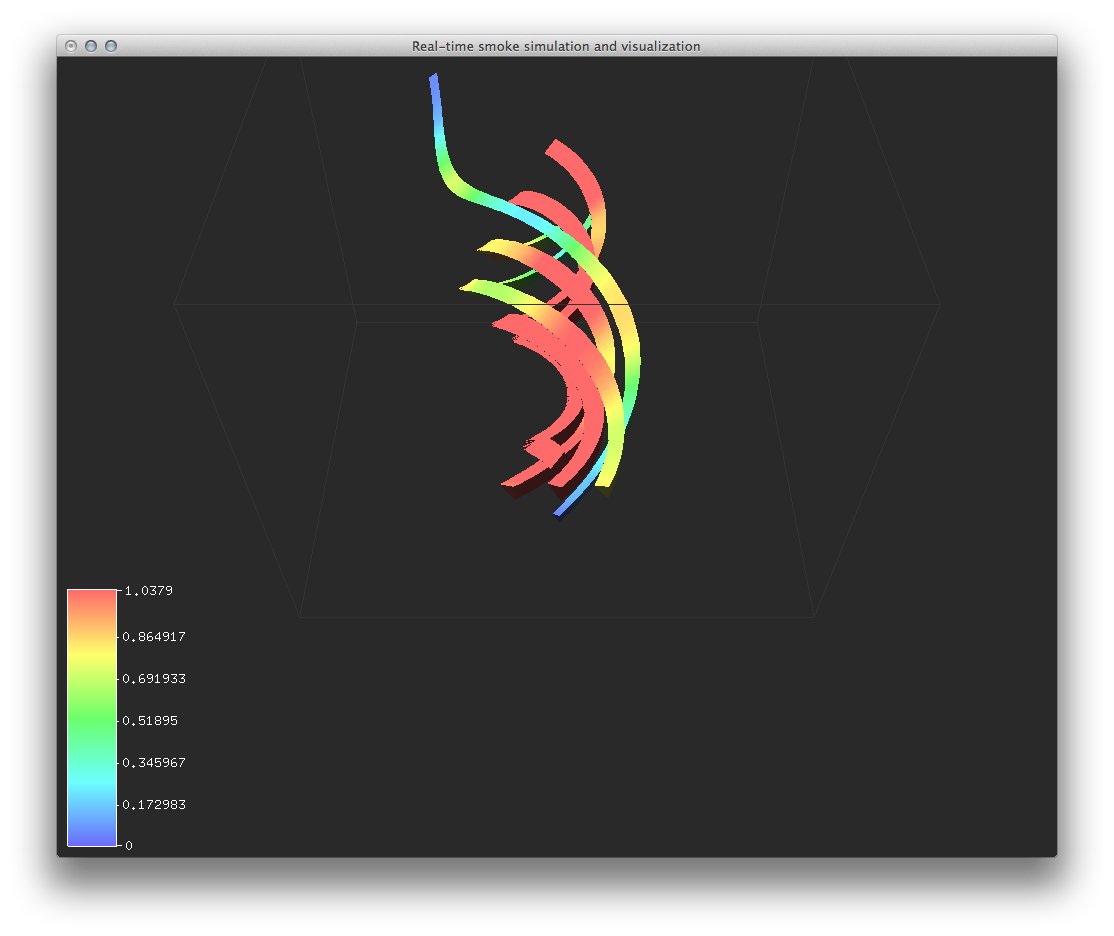
\includegraphics[height=3in]{figures/streamtubes/41flatshading.png}
    \caption{}
    \label{fig:}
\end{minipage}
\end{figure}

